% Metódy inžinierskej práce

\documentclass[10pt,twoside,slovak,a4paper]{article}

\usepackage[slovak]{babel}
%\usepackage[T1]{fontenc}
\usepackage[IL2]{fontenc} % lepšia sadzba písmena Ľ než v T1
\usepackage[utf8]{inputenc}
\usepackage{graphicx}
\usepackage{url} % príkaz \url na formátovanie URL
\usepackage{hyperref} % odkazy v texte budú aktívne (pri niektorých triedach dokumentov spôsobuje posun textu)

\usepackage{cite}
%\usepackage{times}

\pagestyle{headings}

\title{Aplikovanie hier v procese vzdelávania\thanks{Semestrálny projekt v predmete Metódy inžinierskej práce, ak. rok 2022/23, vedenie: Igor Stupavský}} % meno a priezvisko vyučujúceho na cvičeniach

\author{Patrik Drdák\\[2pt]
	{\small Slovenská technická univerzita v Bratislave}\\,
	{\small Fakulta informatiky a informačných technológií}\\
	{\small \texttt{xdrdak@stuba.sk}}
	}

\date{\small 19. október 2022} % upravte


\begin{document}

\maketitle

\begin{abstract}
\ldots
\end{abstract}

\section{Abstrakt}
Tento príspevok rozoberá aplikovanie hier
ako edukačnej pomôcky na príjem informácií ale taktiež interagovanie s nimi,
čo vo výsledku by malo mať pozitívny vplyv na efektivitu učenia sa a samotné
učenie. Použitie týchto hier by malo mať takisto pozitívny vplyv na komunikáciu medzi študentom a pedagógom ako aj medzi študentmi navzájom. Súčasťou príspevku je taktiež zameranie sa na efektivitu používania vzdelávacích hier, to znamená na dosiahnuté výsledky v porovnaní s tými bez použitia týchto hier.


\section{Úvod}

Hra nie je iba pre deti a je známe, že najviac informácií si vieme zapamätať, keď máme z edukácie zážitok a vytvoria v nás pozitívnu emočnú stopu. A o tom využitie herných prvkov v nehernom prostredí práve je. Napriek preukázaným výhodám Serious Games v porovnaní s tradičným e-learningom, využívanie učenia založeného na hrách
v bežnom vzdelávaní je stále veľmi nízke. Zvýšená absorpcia
vyžaduje uľahčenie nasadenia vhodných hier ako typu aktivity
v existujúcich e-learningových platformách. Hlavné ciele gamifikácie sú zlepšenie určitých schopností, zapojenie študentov, optimalizovanie učenie, podporovanie zmeny správania a socializovanie sa. Stimulovaní efektmi, ktoré môžu herné prvky vyvolať, mnohí výskumníci skúmali vplyv gamifikácia vo vzdelávacom kontexte, pričom dosiahli priaznivé výsledky, ako je zvýšenie angažovanosti, pozornosti, vedomostí a spolupráce. Napriek tomu niektoré štúdie ukázali neisté alebo škodlivé výsledky gamifikácie. Zistili, že hodnotenie ovplyvňuje ženy rôznymi spôsobmi a môže viesť k neočakávanému opačnému vplyvu.





\section{Čo je to gamifikácia} 

Z obr.~\ref{f:rozhod} je všetko jasné. 

\begin{figure*}[tbh]
\centering
%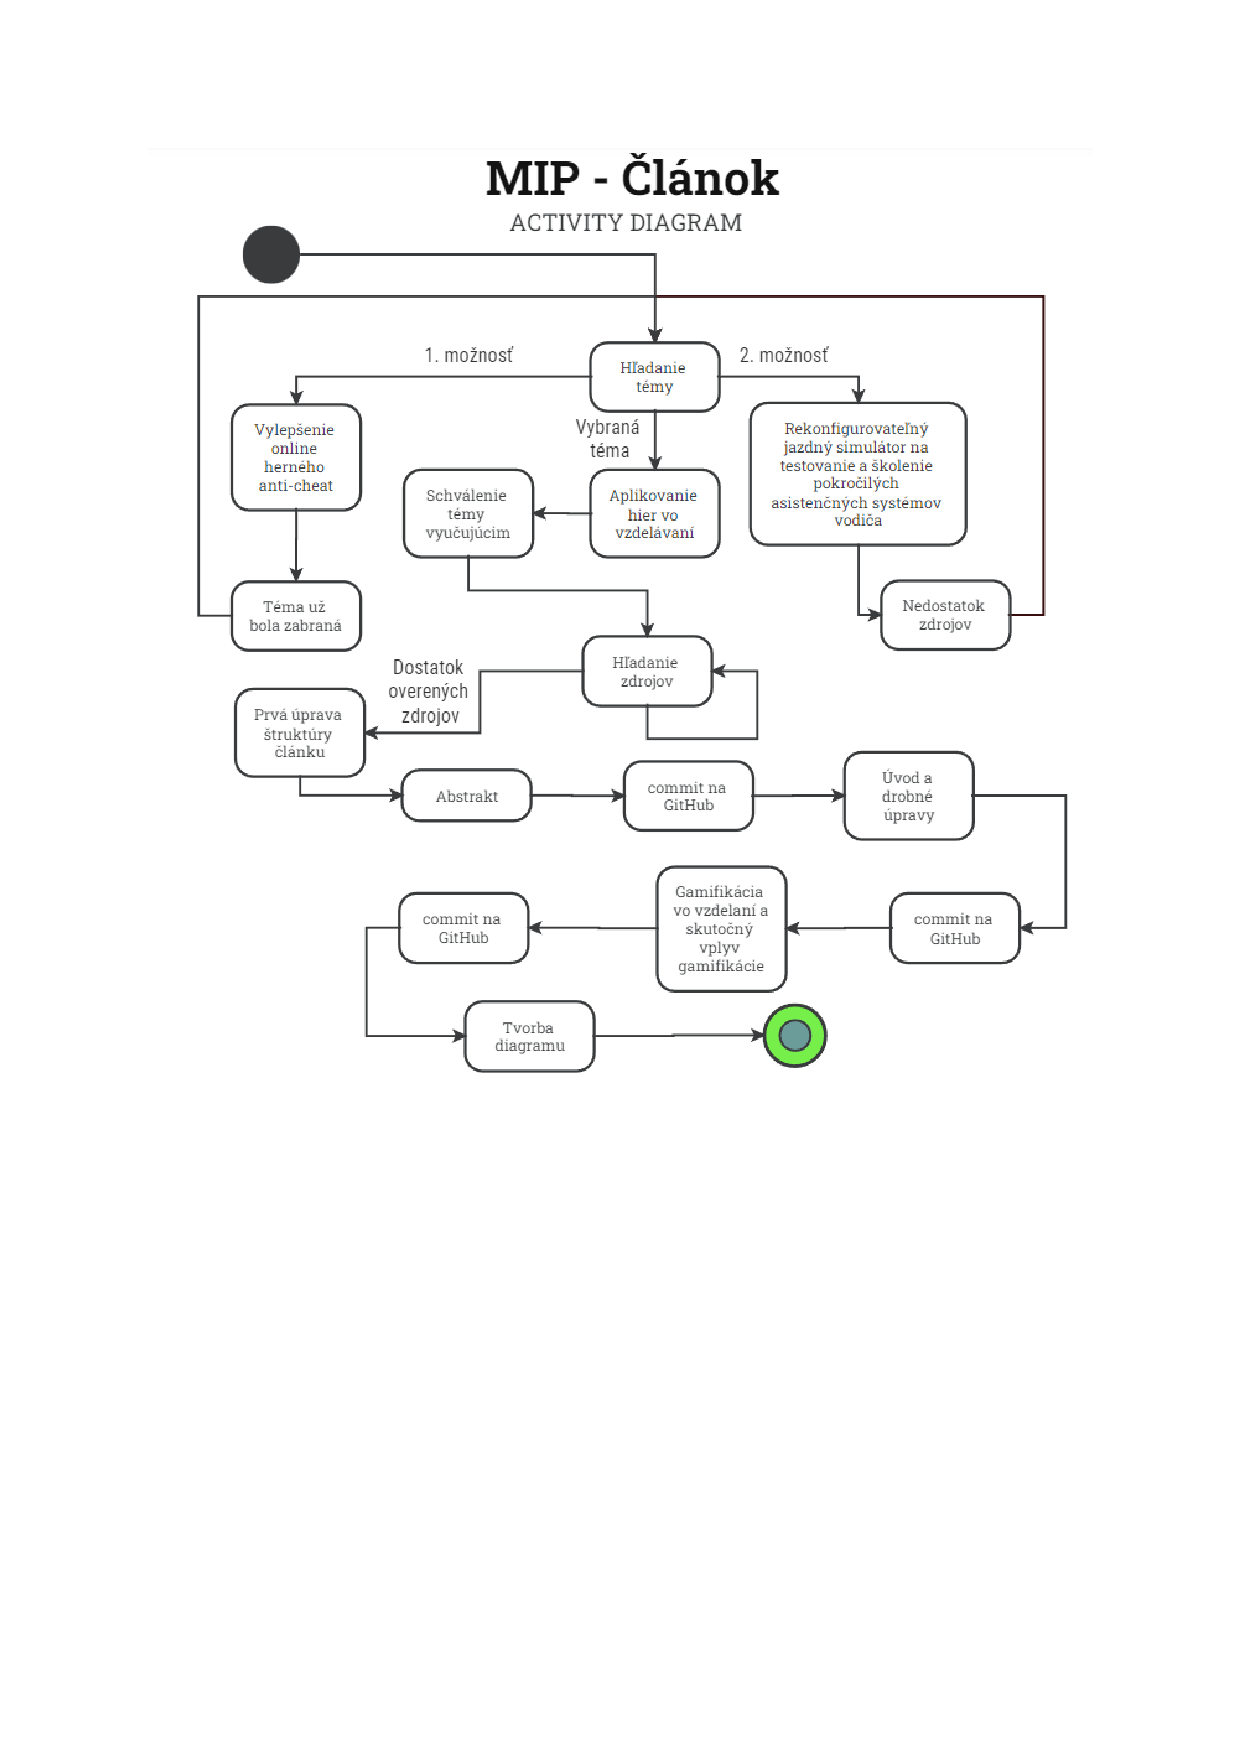
\includegraphics[scale=1.0]{diagram.pdf}
Aj text môže byť prezentovaný ako obrázok. Stane sa z neho označný plávajúci objekt. Po vytvorení diagramu zrušte znak \texttt{\%} pred príkazom \verb|\includegraphics| označte tento riadok ako komentár (tiež pomocou znaku \texttt{\%}).
\caption{Rozhodujúci argument.}
\label{f:rozhod}
\end{figure*}



\section{Iná časť} \label{ina}

Základným problémom je teda\ldots{} Najprv sa pozrieme na nejaké vysvetlenie (časť~\ref{ina:nejake}), a potom na ešte nejaké (časť~\ref{ina:nejake}).\footnote{Niekedy môžete potrebovať aj poznámku pod čiarou.}

Môže sa zdať, že problém vlastne nejestvuje\cite{Coplien:MPD}, ale bolo dokázané, že to tak nie je~\cite{Czarnecki:Staged, Czarnecki:Progress}. Napriek tomu, aj dnes na webe narazíme na všelijaké pochybné názory\cite{PLP-Framework}. Dôležité veci možno \emph{zdôrazniť kurzívou}.


\subsection{Nejaké vysvetlenie} \label{ina:nejake}

Niekedy treba uviesť zoznam:

\begin{itemize}
\item jedna vec
\item druhá vec
	\begin{itemize}
	\item x
	\item y
	\end{itemize}
\end{itemize}

Ten istý zoznam, len číslovaný:

\begin{enumerate}
\item jedna vec
\item druhá vec
	\begin{enumerate}
	\item x
	\item y
	\end{enumerate}
\end{enumerate}


\subsection{Ešte nejaké vysvetlenie} \label{ina:este}

\paragraph{Veľmi dôležitá poznámka.}
Niekedy je potrebné nadpisom označiť odsek. Text pokračuje hneď za nadpisom.

\section{pokus}\input{novy.tex}
\subsection{cccc}



\section{Dôležitá časť} \label{dolezita}




\section{Ešte dôležitejšia časť} \label{dolezitejsia}




\section{Záver} \label{zaver} % prípadne iný variant názvu



%\acknowledgement{Ak niekomu chcete poďakovať\ldots}


% týmto sa generuje zoznam literatúry z obsahu súboru literatura.bib podľa toho, na čo sa v článku odkazujete
\bibliography{literatura}
\bibliographystyle{alpha} % prípadne alpha, abbrv alebo hociktorý iný
\end{document}